\documentclass[journal,10pt]{IEEEtran}
\usepackage{sharina}

\begin{document}
% Inspired by title template from ShareLaTeX Learn; Gubert Farnsworth & John Doe
% Edited by Jon Arnt Kårstad, NTNU IMT
% Edited by Linda Vogel, HTWK
\begin{titlepage}
\vbox{ }
\vbox{ }
\begin{center}
% Upper part of the page


\includegraphics[width=0.40\textwidth]{liverpool.png}\\[1cm]
%\includegraphics[width=0.40\textwidth,left]{Images/HTWK-Fakultaetszusatz_ing_schwarz_de.png}\\[1cm]

\textsc{\LARGE THE UNIVERSITY OF LIVERPOOL}\\[1.5cm]
\textsc{\Large COMP702-MSC Final Project}\\[0.5cm]
\vbox{ }

% Title


\huge \bfseries Visual Spatial Reasoning for Large Language Models\\[0.4cm]


\begin{table}[h]
\large
    \centering
    \begin{tabular}{ll}
        \emph{Author} & Jinlong Liu \\
        \emph{Student ID} & 201678181\\
        \emph{Supervisor} &  Frank Wolter \\
        \emph{Second Marker} &  Boris Konev \\
    \end{tabular}
\end{table}

\vfill
% Bottom of the page
{\large \today}
\end{center}
\end{titlepage}
\section{Project Description}

In recent years, Large Language Models (LLMs) have transformed the field of Natural Language Processing (NLP) with their impressive achievements. These models, which have been trained on extensive amounts of text data, have proven to be highly effective in solving various NLP tasks, like translating languages, answering questions, and generating text. Their ability to understand and create text that resembles human language has been truly remarkable and easy to appreciate.

However, despite their proficiency in many linguistic tasks, LLMs have faced challenges when it comes to Spatial Reasoning. Unlike tasks that focus solely on language, Spatial Reasoning involves comprehending and manipulating visual and spatial information. To shed light on this limitation, I plan to conduct an experiment using popular LLMs like GPT-4\cite{peng2023instruction}. The main goal will be to test how well they can handle Visual Spatial Reasoning, which is important for understanding the relationships between objects in visual content.

The experiment will center around a commonly used task called Visual Question Answering (VQA). This task requires machines to answer questions based on provided images. For example, when given an image showing different objects, the machine will be given inquiries such as "What is the spatial relationship between object A and object B?". By designing carefully constructed tests like these, we can assess the level of Spatial Reasoning ability demonstrated by LLMs in an easy-to-understand manner.

Through evaluating their performance in VQA and their capacity to comprehend and reason about spatial relationships in visual content, we can gain valuable insights into the Spatial Reasoning capabilities of LLMs. These findings will not only enhance our understanding of the strengths and limitations of these models but also pave the way for further advancements in NLP. This progress will bring us closer to developing more comprehensive and versatile language models that are accessible and easy to work with.

\section{Aims and Objectives}
In this section, we will provide a clear outline of the aims and objectives of this project. The aims represent the overarching goals that we aim to achieve, while the objectives outline the specific steps and milestones that will be undertaken to fulfill these goals. The aims and objectives of this project are outlined below:
\subsection{Aims}
\begin{enumerate}
    \item To investigate the Spatial Reasoning abilities of Large Language Models (LLMs), specifically focusing on their performance in Visual Question Answering (VQA) tasks.
    \item To understand the limitations and challenges faced by LLMs in comprehending and reasoning about spatial relationships in visual content.
    \item To assess the current state of Spatial Reasoning capabilities in leading LLMs, then compare with elder models and explore their improvement in this domain. Besides, to identify potential avenues for enhancing LLMs' Spatial Reasoning abilities.
\end{enumerate}
\subsection{Objectives}
\begin{enumerate}
    \item Design and develop a comprehensive experimental framework for evaluating LLMs' Spatial Reasoning abilities in VQA tasks.
    \item Curate a diverse dataset of visual stimuli and corresponding questions that require spatial reasoning skills to answer accurately.
    \item Conduct systematic experiments using the prepared dataset and modified LLMs to assess their performance and measure their level of Spatial Reasoning competence.
    \item Analyze the experimental results to identify patterns, trends, and challenges in LLMs' Spatial Reasoning capabilities.
    \item Provide insights into the strengths and limitations of current LLMs for Spatial Reasoning tasks, based on the experimental findings.
    \item Suggest potential avenues for enhancing LLMs' Spatial Reasoning abilities, such as incorporating multimodal information or novel architectural modifications.
    \item Contribute to the existing body of knowledge in the field of NLP by advancing our understanding of LLMs' Spatial Reasoning abilities and their implications for future research and development.
\end{enumerate}

In summary, this project aims to investigate the Spatial Reasoning abilities of LLMs, specifically in VQA tasks, by designing experiments, analyzing results, and providing insights for improvement. By achieving these objectives, the project will contribute to the advancement of NLP and enhance our understanding of LLMs' capabilities in comprehending and reasoning about spatial relationships in visual content.

\section{Key Literature and Background Reading}
Spatial Reasoning ability is a crucial aspect of human intelligence, enabling us to understand and manipulate spatial information. It is a fundamental skill that allows us to navigate the world around us, comprehend visual content, and solve spatial problems. It is also a goal to be achieved by Artificial Intelligence (AI) systems, as it is a key component of human-level intelligence. At first, the representation of spatial knowledge having a different way of thinking from the representation of language knowledge, it is difficult to combine the two. However, with the development of deep learning, the combination of the two has become possible.

For LLMs, Spatial Reasoning encompasses several key aspects, including (i) mereotopology, (ii) direction and orientation, (iii) size, (iv) distance, and (v) shape, as discussed by Cohn et al. (2008) in their qualitative analysis \cite{cohn2008qualitative}. To assess LLMs' performance in Spatial Reasoning, Cohn et al. (2023) developed a comprehensive Spatial Reasoning test that incorporates basic spatial relations (such as parthood, rotation, and direction), size, shape, location, affordances, object interaction, and object permanence \cite{cohn2023dialectical}. Their findings revealed inconsistencies in LLMs' responses to the same question during continuous sessions, indicating that LLMs struggle with maintaining consistency in Spatial Reasoning tasks.

In a related study by Lin et al. (2023), a test was devised to evaluate LLMs' Spatial Reasoning abilities with a focus on mathematical representation of questions \cite{lin2023using}. Their research demonstrated that while LLMs may not excel at directly answering spatial questions, they exhibit proficiency in transforming questions into mathematical forms based on user demands.

Moreover, Borji (2023) proposed a failure task category for ChatGPT, within which Spatial Reasoning was highlighted \cite{borji2023categorical}. In this task, the researcher provided a grid description and asked the model to find a path from a start point to an end point. However, the model failed to answer the question accurately, highlighting its limitations in Spatial Reasoning tasks.

Collectively, these studies shed light on the challenges LLMs face when it comes to Spatial Reasoning, including inconsistencies in responses, struggles with direct spatial question answering, and difficulties in solving specific spatial tasks like path finding. 

One important aspect to consider is Visual Spatial Reasoning (VSR) and its relevance in the context of Visual Language Models (VLMs), which is a distinct topic from LLMs. It is worth highlighting some related research in this field.

Researchers have dedicated efforts to assess the ability of VLMs in comprehending commonsense spatial reasoning. Visual Question Answering (VQA) tasks have been employed to evaluate the performance of VLMs in answering questions that involve spatial relationships between objects depicted in images\cite{7410636}. Consequently, various benchmarks and question sets have been developed to specifically evaluate the spatial reasoning capabilities of VLMs.

For instance, Liu et al. (2022) constructed a dataset consisting of over 10,000 text-image pairs, encompassing 66 types of spatial relations \cite{liu2022visual}. They evaluated the performance of both human subjects and VLMs on this dataset, revealing that VLMs still lag behind humans in this task. Additionally, other benchmarks such as GQA \cite{hudson2019gqa}, AGQA \cite{grunde2021agqa}, Compositional Visual Relations Dataset \cite{zerroug2022benchmark}, VALSE \cite{parcalabescu2021valse}, Liu et al. (2021) \cite{liu2022things}, and SpartQA \cite{mirzaee2021spartqa} have been developed to further gauge the spatial reasoning capabilities of VLMs.

These benchmarks and datasets serve as valuable tools to assess the progress and limitations of VLMs in the realm of spatial reasoning and they have such things in common: (i) they are all based on commonsense spatial reasoning, (ii) they all focus on VLMs, and (iii) they all given some bound words to the model to help it understand the spatial relations. However, in my research, I will focus on LLMs and their Spatial Reasoning capabilities, which is a distinct topic from VLMs. 


\section{Development and Implementation Summary}
This project aims to investigate the Visual Spatial Reasoning capabilities of LLMs, specifically focusing on their performance in VQA tasks. So the development and implementation of this project will be divided into these parts:

\subsection{Probelm Identification}
The main problem of this project is to investigate the Spatial Reasoning abilities of LLMs, specifically focusing on their performance in VQA tasks. So the first step is to identify the problem and the research questions. The research questions are as follows:
\begin{enumerate}
    \item What are the Spatial Reasoning abilities of LLMs?
    \item What are the limitations and challenges faced by LLMs in comprehending and reasoning about spatial relationships in visual content?
    \item What is the current state of Spatial Reasoning capabilities in leading LLMs?
    \item What are the potential avenues for enhancing LLMs' Spatial Reasoning abilities?
\end{enumerate}

\subsection{Experiment Design}
For the experimental stage, the workflow can be visualized as depicted in Figure \ref{fig:workflow}. The experiment is divided into three distinct parts, each serving a specific purpose:
\begin{enumerate}
    \item \textbf{Prepare Stage}
    \subitem During this stage, the primary objective is to gather a diverse collection of images that contain various spatial relations. These images can be sourced from the internet or generated using appropriate tools. For this project, the dataset will consist of a combination of an existing benchmark proposed by Liu et al. (2022) \cite{liu2022visual}.
    Another crucial aspect is the question set, which will be divided into two parts:
    (i) Questions discussing the spatial relationships between objects depicted in the images.
    (ii) Questions requiring the reasoning steps behind the previous answers.
    \item \textbf{Experiment Stage}
    \subitem The focus of this stage is to test different versions of Large Language Models (LLMs) using the prepared dataset and question set. The LLMs will be evaluated based on two factors:
    (i) Different sizes of LLMs.
    (ii) Different pre-training methods of LLMs.
    The experiment will involve running the LLMs on the prepared dataset, recording the results, and analyzing their performance. And all testing models will be GPT models, including from GPT-3.5 tubor to GPT-4-0612.
    \item \textbf{Analysis and Evaluation Stage}
    \subitem In this stage, the emphasis is on analyzing the performance of the different versions of LLMs using the prepared dataset. The analysis will primarily consider two aspects:
    (i) The accuracy of the answers provided by the LLMs.
    (ii) The reasoning steps generated by the LLMs.
    Based on the accuracy, the effectiveness and capability of the LLMs in spatial reasoning can be evaluated and compared. By examining the reasoning steps, any limitations and challenges faced by LLMs in comprehending and reasoning about spatial relationships in visual content can be identified.
\end{enumerate}

Through this systematic workflow, the experiment aims to assess the performance and capabilities of various versions of LLMs in spatial reasoning tasks. The analysis and evaluation stage provide insights into the strengths, weaknesses, and potential areas for improvement in LLMs' understanding and reasoning abilities pertaining to spatial relationships in visual content.

\subsection{Code Implementation}
There is no code implementation in this project. All the experiments will be conducted on the website of OpenAI. The code of this project will be written in Python, and the code will be used to prepare the dataset and question set, and to analyze the results of the experiment.

\begin{figure}[htbp]
    \centering
    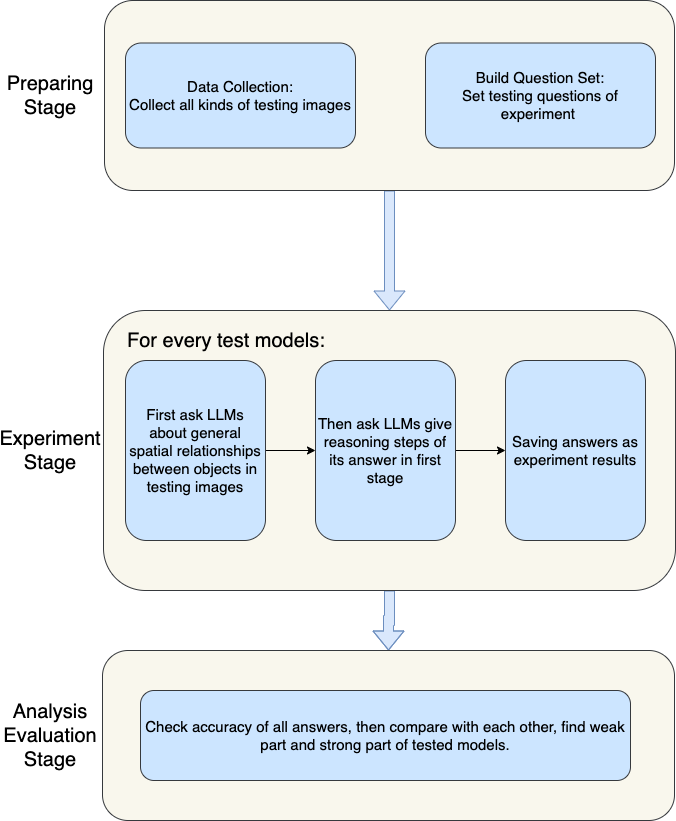
\includegraphics[width=0.8\linewidth]{./pic/workflow.drawio.png}
    \caption{Workflow of the experiment}
    \label{fig:workflow}
\end{figure}

\section{User Interface Mockup}
For this project, there is no user interface mockup. All the experiments will be conducted on the website of OpenAI. The code of this project will be written in Python, and the code will be used to prepare the dataset and question set, and to analyze the results of the experiment.

\section{Data Sources}
The data utilized in this project will be divided into two main parts: the dataset and question set, and the answers generated by the Large Language Models (LLMs).

For the dataset and question set, a combination of existing benchmarks proposed by Liu et al. (2022) \cite{liu2022visual} and self-generated images will be used. The images in the dataset will encompass real-world objects along with 2D shapes, ensuring a diverse range of spatial relationships to be examined. The benchmark images are extracted from the COCO 2017 dataset \cite{lin2014microsoft}, which is an open-source dataset widely used in computer vision research. It is important to note that the usage of the COCO dataset has been granted full permission for this project.

As for the second part, the answers generated by the LLMs will be stored in a text file. The answers will be generated using the OpenAI website, which provides a platform for executing queries and obtaining responses from the language model. The generated answers can be conveniently downloaded as a text file from the website or saved directly on the platform.

By utilizing this comprehensive data setup, incorporating a combination of benchmark images and self-generated content, along with leveraging the power of LLMs to generate answers, the project aims to provide an extensive and diverse set of data for analysis and evaluation. The combination of the benchmark dataset and the generated answers will enable the project to assess the performance and capabilities of the LLMs in spatial reasoning tasks accurately.

It is important to ensure adherence to proper data usage policies, including obtaining necessary permissions for the benchmark dataset and complying with any licensing or attribution requirements associated with the dataset. This approach ensures the project's integrity and ethical practices while utilizing publicly available data resources for research purposes.

\section{Testing}

\section{Evaluation}
\section{Ethical Considerations}
As researchers and developers explore the capabilities of LLMs in visual spatial reasoning, it is crucial to consider and address several ethical considerations associated with this technology. These considerations are necessary to ensure responsible and ethical use of LLMs in the context of visual spatial reasoning. Some key ethical considerations include:
\begin{enumerate}
    \item Bias and Fairness: LLMs are trained on vast amounts of data, and if the training data contains biases, the models can inadvertently perpetuate and amplify those biases. Care should be taken to identify and mitigate biases related to spatial relationships, objects, or cultural aspects in the training data. Fairness and inclusivity should be prioritized to avoid marginalization or discrimination based on race, gender, socioeconomic status, or any other protected characteristics.
    \item Data Privacy and Security: When collecting or using datasets for visual spatial reasoning tasks, it is essential to respect privacy rights and comply with data protection regulations. Any personally identifiable information (PII) should be handled with care, and proper anonymization techniques should be employed to protect the privacy of individuals represented in the data. Additionally, robust security measures should be implemented to prevent unauthorized access to sensitive data.
    \item Informed Consent: If human subjects are involved in data collection or evaluation processes, informed consent should be obtained. Participants should be fully informed about the purpose of the study, the data collection methods, and any potential risks or implications associated with their participation. Participants should have the freedom to withdraw their consent at any point during the study.
    \item Transparency and Explainability: LLMs often operate as black boxes, making it challenging to understand how they arrive at their answers or reasoning steps. It is important to develop methods and techniques that enhance the transparency and explainability of LLMs' decision-making processes in visual spatial reasoning. This helps build trust and allows users to better understand the models' behavior and potential limitations.
    \item Human-AI Collaboration: While LLMs can provide valuable insights and assist in visual spatial reasoning, it is crucial to acknowledge the importance of human expertise and maintain a human-centric approach. LLMs should be viewed as tools to augment human capabilities rather than replacing human decision-making or responsibility. Collaboration between humans and AI should be encouraged to ensure that decisions made based on LLM-generated outputs are critically evaluated and aligned with ethical standards.
    \item Accountability and Governance: As LLMs become more sophisticated, it is important to establish accountability mechanisms and governance frameworks to address any potential risks or unintended consequences. This may include adopting standards, guidelines, or regulatory frameworks specific to the development and deployment of LLMs in visual spatial reasoning applications. Responsible and ethical practices should be promoted throughout the entire lifecycle of LLM development and deployment.
    \item 
\end{enumerate}
These ethical considerations serve as a starting point for ensuring the responsible and ethical use of LLMs in visual spatial reasoning. It is crucial for researchers, developers, and stakeholders to actively engage in ongoing discussions, collaborate with interdisciplinary teams, and adhere to ethical guidelines to mitigate potential harms and maximize the benefits of this technology in a responsible manner.

\section{Project Plan}
The project timeline and task allocation are visually represented in Figure \ref{fig:gantt}, showcasing the specific Gantt chart. The project is organized into four distinct stages, each comprising multiple tasks aimed at achieving the project objectives. The stages and their corresponding tasks are outlined below:
\begin{enumerate}
    \item Literature Review
    \subitem This stage focuses on conducting an extensive literature review to gain a comprehensive understanding of the project domain. It is divided into three tasks:
    \begin{itemize}
        \item Literature review: Conduct a thorough review of relevant research, technologies, and best practices in the field.
        \item Problem identification: Identify the key challenges and opportunities that the project aims to address.
        \item Experiment design: Plan and design the experimental framework and methodologies for subsequent stages.
    \end{itemize}
    \item Build Dataset
    \subitem In this stage, the focus is on creating the dataset and question set required for the experiments. It involves two tasks:
    \begin{itemize}
        \item Prepare dataset: Collect or curate a dataset comprising a combination of existing benchmark images and self-generated images.
        \item Prepare question set: Design and develop a set of questions that encompass various spatial relationships and reasoning scenarios.
    \end{itemize}
    \item Experiment Stage
    \subitem The experiment stage involves executing the designed experiments using the created dataset and question set. This stage is divided into two tasks:
    \begin{itemize}
        \item Run experiment: Implement the experiments using the selected Large Language Models (LLMs) and the prepared dataset and question set.
        \item Record results: Collect and document the results obtained from the experiments, ensuring comprehensive record-keeping.
    \end{itemize}
    \item Analysis and Evaluation Stage
    \subitem In this stage, the focus is on analyzing and evaluating the results obtained from the experiments. This stage comprises two tasks:
    \begin{itemize}
        \item Analyze results: Perform a detailed analysis of the experimental outcomes, considering the accuracy of answers and the reasoning steps generated by the LLMs.
        \item Evaluate results: Assess the performance and effectiveness of the LLMs in spatial reasoning, identify limitations, and recognize challenges faced by the models.
    \end{itemize}
    \item Final Report
    \subitem The final stage involves documenting the project outcomes in a report and preparing a presentation. It is divided into two tasks:
    \begin{itemize}
        \item Write report: Compile all the findings, methodologies, and conclusions into a comprehensive report that highlights the project's objectives, methodology, and results.
        \item Write presentation: Create a visually engaging presentation summarizing the project's key aspects, including objectives, methodology, results, and conclusions.
    \end{itemize}
\end{enumerate}

By following this well-structured project plan, the project aims to ensure efficient task allocation, timely execution, and a systematic approach towards achieving the project objectives. The defined stages and tasks provide a clear roadmap for project completion and successful delivery of the intended outcomes.
\begin{figure*}[htbp]
    \centering
    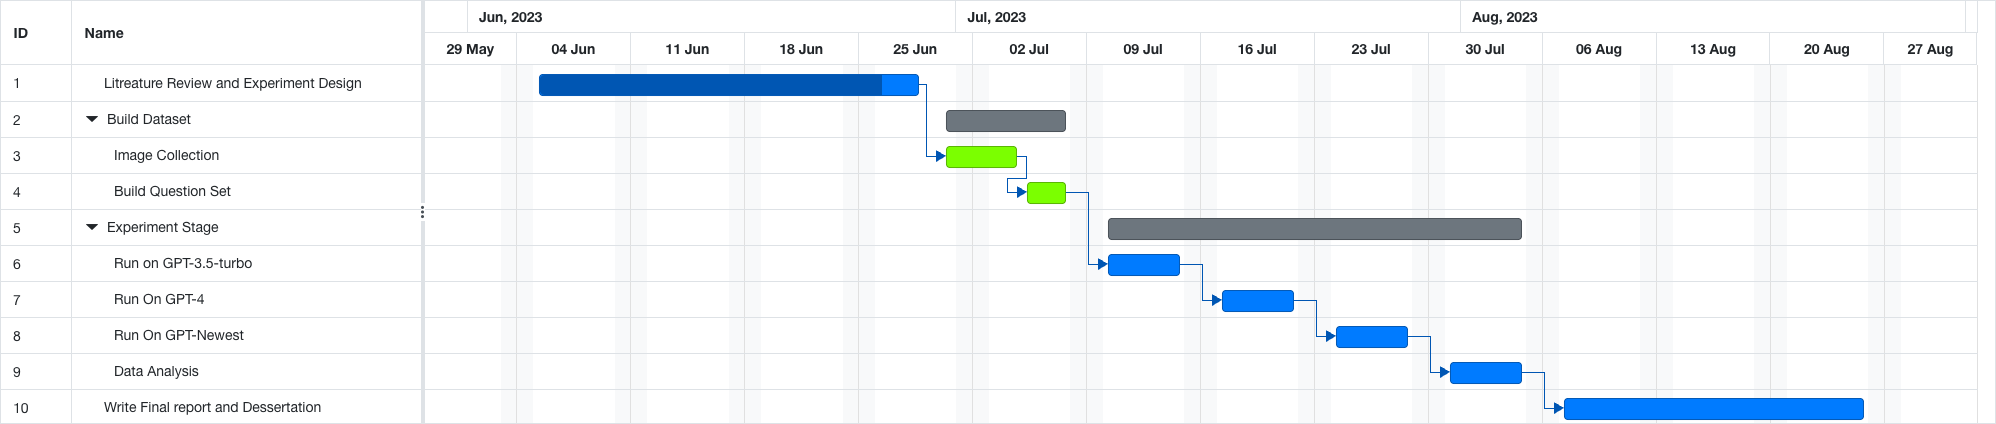
\includegraphics[width=0.8\linewidth]{./pic/Gnatt.png}
    \caption{Gantt Chart}
    \label{fig:gantt}
\end{figure*}

\section{Risks and Contingency Plans}

\bibliographystyle{IEEEtran}
\bibliography{mybib}

\end{document}